\section{Tests de performance}
\subsection{Génération de chemins et circuits hamiltoniens}
Dans ce chapitre, nous allons parler des résultats obtenus avec les algorithmes de génération ce chemins et circuits.
\subsubsection{Chemins et circuits avec l'heuristique de Warnsdorff}
Pour trouver des chemins, le départage aléatoire de candidats de même poids sous l'heurisitque de Warnsdorff fonctionne bien avec de "petits échiquiers carrés". En dessous de 50 cases de côté, l'heuristique permet de trouver un chamin à presque tous les coups. Et ce, dans des temps inférieurs à la seconde. Cependant, pour de plus grands échiquiers, l'heuristique est bien moins fiable. Le caractère aléatoire du départage necessite parfois plusieurs générations pour trouver un chemin valide. La figure ~\ref{WanrsdorffCarreReussite} représente l'évolution de l'efficacité de l'heuristique. Pour chaque taille de tableau, 100 générations de chemins ont été effectuées. La proportion de chemins valides est représentée sur le graphique. ON observe effectivement qu'au delà de 50 cases de côté, l'efficacité dégringole.

\begin{figure}[h]
\begin{center}
   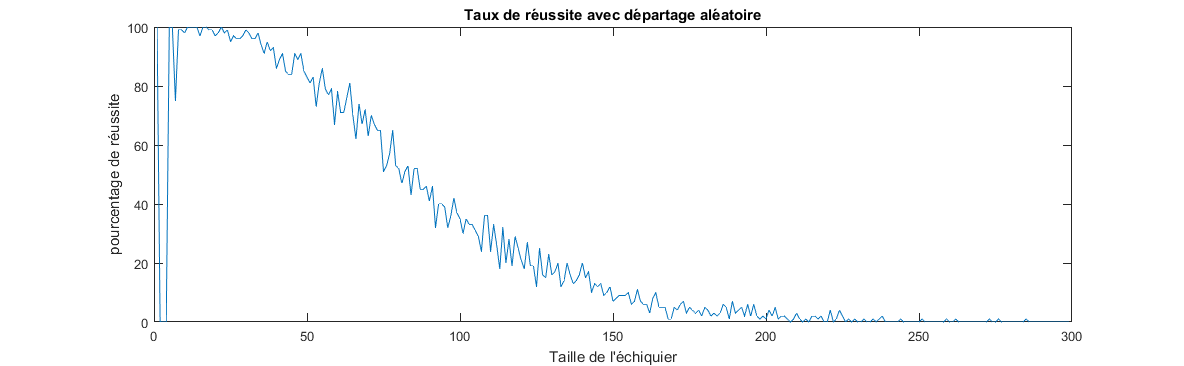
\includegraphics[scale=0.6]{img/WarnsdorffTauxReussiteCarre.png} 
   \caption{\label{WanrsdorffCarreReussite} Taux de réussite pour la génération de chemins hamiltoniens sur échiquiers carrés avec l'heurisitque de Warnsdorff}
   \end{center}
\end{figure}

Des tests ont également été faits avec des échiquiers rectangulaires, de taille n*m, n<=m. La figure ~\ref{WanrsdorffRectangleReussite} présente un graphique du taux de réussite. Chaque échiquier testé est représenté avec son nombre de lignes en abscisse et son nombre de colonnes en ordonnée. Si la couleur de l'échiquier est jaune, le taux de réussite est proche de 100\%. Si elle est bleue, le taux de réussite est proche de 0\%. Nous pouvons observer que les résultats les plus satisfaisants sont pour les échiquiers avec m et n inférieurs à 50. De plus, plus m et n sont proches, plus les résultats sont concluants. Cette observation n'est pas surprenante si on se fie aux résultats sur les échiquiers carrés.

\begin{figure}[h]
\begin{center}
   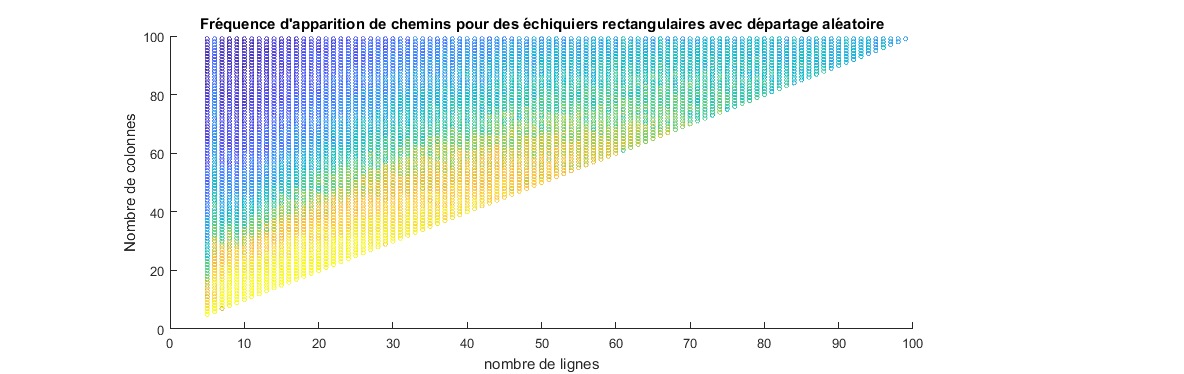
\includegraphics[scale=0.6]{img/WarnsdorffTauxReussiteRectangle.png} 
   \caption{\label{WanrsdorffRectangleReussite} Taux de réussite pour la génération de chemins hamiltoniens sur échiquiers rectangulaires avec l'heurisitque de Warnsdorff}
   \end{center}
\end{figure}

Nous avons également tenté de trouver des circuits hamiltoniens avec le départage aléatoire sur des échiquiers carrés. Nous étions partis du principe que comme le circuit est une forme particulière du chemin, il y avait une probabilité non nulle de générer des circuits. La figure ~\ref{CircuitCarre} présente ces résultats. Pour chaque dimension d'échiquier, nous avons réalisé 100 000 essais, et repis la proportions de circuits valides. Il apparait sans trop de surprise que les résultats obtenus sont très peu concluants. Pour un échiquier de 8 cases de côté, seuls 20 essais sur 100000 furent valides. 

\begin{figure}[h]
\begin{center}
   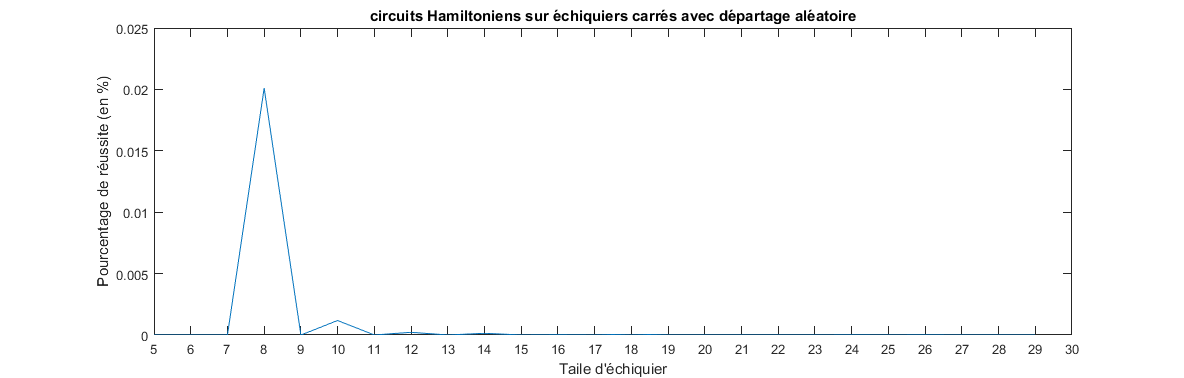
\includegraphics[scale=0.6]{img/circuitCarre.png} 
   \caption{\label{CircuitCarre} Taux de réussite pour la génération de circuits hamiltoniens sur échiquiers carrés avec l'heurisitque de Warnsdorff}
   \end{center}
\end{figure}

\subsubsection{chemins hamiltoniens avec l'algorithme de Squirrel}
Les tests effectués avec l'algorithme de Squirrel sont plus satisfaisants qu'avec le départage aléatoire. Squirrel définit son algorithme comme fonctionnel pour tout échiquier carré de plus de 112 cases de côté. Il propose également des permutations de l'ordre de parcours efficaces pour des échiquiers de taille inférieure à 112. Nous avons effectué nos tests uniquement avec l'algorithme originel. Et celui-ci s'est montré fiable à tous les coups pour tout échiquier de plus de 5 carrés de côté. A une exception, lorsqu'il y a 74 cases de côté. Dans ce cas là, l'algorithme rate à tous les coups. Il serait donc intéressant de tester une permutaiton fonctionnelle pour cette dimension d'échiquier. 

La figure ~\ref{TempsSquirrel} montre les temps de calcul obtenus avec l'algorithme de Squirrel pour des échiquiers avec 5 <= n <= 10000. L'évolution des temps de calcul est légèrement supérieure à la complexité $\theta(n^2)$ annoncée. Cela est certainement dû à notre implémentation en C.
\begin{figure}[h]
\begin{center}
   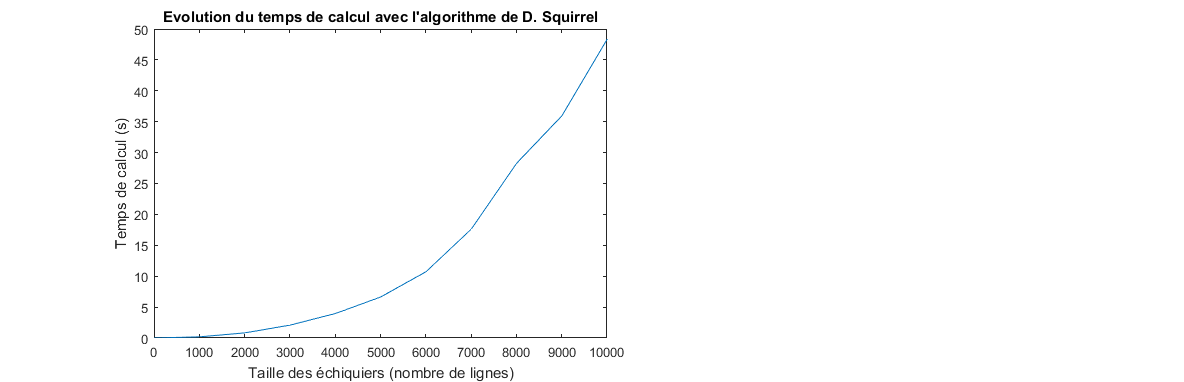
\includegraphics[scale=0.6]{img/TempsSquirrel.png} 
   \caption{\label{TempsSquirrel} Temps de calcul mesurés avec l'algorithme de Squirrel}
   \end{center}
\end{figure}

\subsubsection{Algorithme de Shun-Shii}
Il n'y a pas grand chose à rajouter sur l'implémentation de cet algorithme. Celui-ci trouve un chemin hamiltonien pour tout échiquier de taille 3*m. Si tant est qu'un chemin existe, conformément au théorème de Schwenk. La complexité est similaire à celle de l'algorithme de Squirrel.